
\documentclass[border=10pt]{standalone}
\usepackage{pgfplots}
\pgfplotsset{compat=1.18}
\begin{document}
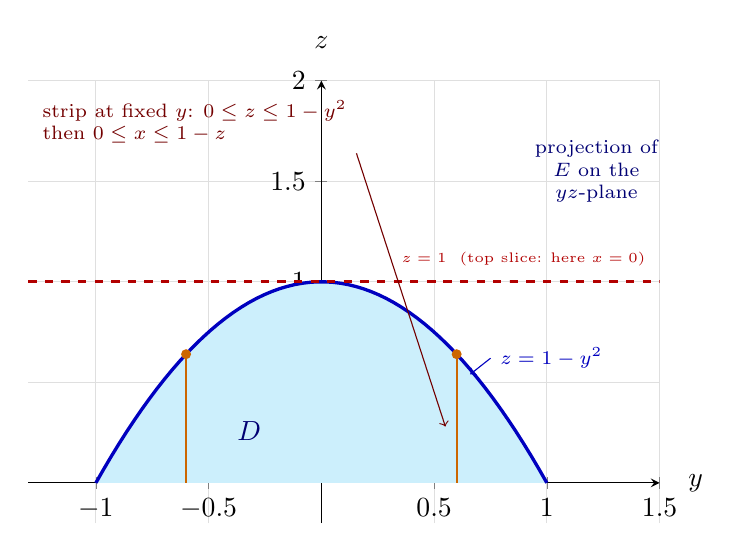
\begin{tikzpicture}
\begin{axis}[
    width=9.6cm, height=7.2cm,
    xlabel={$y$}, ylabel={$z$},
    xmin=-1.30, xmax=1.50, ymin=-0.20, ymax=2.00,
    axis lines=middle, grid=major, grid style={gray!25},
    xlabel style={at={(ticklabel* cs:1.03)}, anchor=west},
    ylabel style={at={(ticklabel* cs:1.05)}, anchor=south},
    samples=60, domain=-1:1, no marks]

  % shaded projection D  (region 0 <= z <= 1-y^2)
  \addplot+[fill=cyan!20, draw=none] {1-x^2} \closedcycle;

  % parabola z = 1 - y^2
  \addplot+[very thick, blue!75!black] {1-x^2};
  \node[blue!75!black, font=\scriptsize] (plbl) at (axis cs:1.02,0.62) {$z=1-y^2$};
  \draw[->, blue!75!black, thin] (plbl.west) -- (axis cs:0.66,0.54);

  % top slice z = 1
  \addplot+[dashed, red!70!black, very thick, domain=-1.30:1.50] {1};
  \node[red!70!black, font=\tiny, anchor=south east] at (axis cs:1.48,1.03)
      {$z=1$\ \ (top slice: here $x=0$)};

  % vertical strips at fixed y
  \draw[orange!80!black, thick] (axis cs:-0.6,0) -- (axis cs:-0.6,0.64);
  \fill[orange!80!black] (axis cs:-0.6,0.64) circle (1.8pt);
  \draw[orange!80!black, thick] (axis cs:0.6,0) -- (axis cs:0.6,0.64);
  \fill[orange!80!black] (axis cs:0.6,0.64) circle (1.8pt);

  \node[black!55!red, font=\scriptsize, align=left, anchor=north west] (txt) at (axis cs:-1.28,1.95)
      {strip at fixed $y$:  $0\le z\le 1-y^2$\\ then $0\le x\le 1-z$};
  \draw[->, black!55!red, thin] (txt.south east) -- (axis cs:0.55,0.28);

  \node[blue!45!black, font=\bfseries] at (axis cs:-0.32,0.26) {$D$};
  \node[blue!45!black, font=\scriptsize, align=center] at (axis cs:1.22,1.55)
      {projection of\\ $E$ on the\\ $yz$-plane};
\end{axis}
\end{tikzpicture}
\end{document}
